\subsection{Fundamentals}

Before presenting the details on the \lstinline|SimEntity| interface,
we take the time to summarize the fundamental concepts in
\lstinline|jsimulation| and \lstinline|jqueues|:
\begin{itemize}
	\item The \lstinline|Java| package named \lstinline|jsimulation|
	is a library for (single-threaded) discrete-event simulation.
	\item The \lstinline|Java| package named \lstinline|jqueues|
	is a library for (single-threaded) discrete-event simulation
	of queueing systems.
	The library depends on \lstinline|jsimulation|.
	\item In order to perform discrete event simulations,
	an event list is needed, on which events can be scheduled.
	The event list maintains an ordering of the events it contains
	in non-decreasing simulation time.
	Typically, a single instance of an event list is used
	throughout the entire simulation study.
	The corresponding (abstract) types
	for event lists and events are defined in \lstinline|jsimulation|,
	and named \lstinline|SimEventList| and \lstinline|SimEvent|, respectively.
	This package also provides a reasonable implementation for
	a \lstinline|SimEventList| named \lstinline|DefaultSimEventList|.
	\item On a \lstinline|SimEventList|, all scheduled \lstinline|SimEvent|s are
	unique; you cannot schedule a \lstinline|SimEvent| more than once
	on a single \lstinline|SimEventList|.
	Typically, \lstinline|SimEvent|s are created and scheduled through
	various utility methods.
	\item The time at which a \lstinline|SimEvent| is scheduled,
	is kept on the \lstinline|SimEvent| itself,
	and available though the \lstinline|SimEvent.getTime| method.
	Once scheduled, you cannot change the time of a \lstinline|SimEvent|.
	You can, however, reschedule it at a different time
	through the \lstinline|SimEventList.reschedule| method.
	\item It is perfectly legel if multiple \lstinline|SimEvent|s are scheduled
	at the same time.
	On a \lstinline|DefaultSimEventList|, they are processed in random order.
	\item With each \lstinline|SimEvent|, an action is associated that determines
	what to do when the event is processed by the event list.
	The generic type in \lstinline|jsimulation| is \lstinline|SimEventAction|.
	Unlike \lstinline|SimEvent|s, \lstinline|SimAction| need not be unique
	on the event list, and can be shared among different events.
	\item Once sufficient events have been scheduled,
	a simulation experiment starts by running or processing
	the event list.
	In \lstinline|jsimulation|,
	you can run the \lstinline|SimEventList| until it is exhausted
	of events through the \lstinline|SimEventList.run| method,
	until it has reached a specific simulation time
	through the \lstinline|SimEventList.runUntil| method,
	or on an event-by-event basis through \lstinline|SimEventList.runSingleStep|.
	\item A \lstinline|SimEventList| keeps a notion of simulation time.
	It is available through \lstinline|SimEventList.getTime|.
	While running,
	this is always the scheduled time of the current event being processed.
	When not, it is always smaller than or equal to the time
	on the first scheduled \lstinline|SimEvent|.
	\item You cannot schedule (at the risk of an \lstinline|Exception|)
	a \lstinline|SimEvent| with time
	strictly smaller than the current simulation time
	on the \lstinline|SimEventList|.
	\item Event may be scheduled simultaneously,
	in which case their order of processing is {\em random}.
	\item Events may be scheduled at $t=-\infty$ and $t=+\infty$.
	\item The \lstinline|SimEventList.reset| and \lstinline|SimEventList (double)|
	methods reset the event list,
	meaning all scheduled \lstinline|SimEvent|s are removed from the list,
	and the time on the event list is set to its default time (first method)
	or given time.
	The typical use case of these methods is running the simulation again
	(for instance, for variance-reduction purposes).
	You cannot invoke either method while the event list is being processed,
	at the risk of an \lstinline|Exception|.
	\item In simulation of queueing systems,
	the center of attention is a simulation entity,
	an object with a state subject to (the actions of) simulation events.
	\item In \lstinline|jqueues|, simulation entities are represented
	as \lstinline|SimEntity| objects.
	In the present release,
	a \lstinline|SimEntity| is either a \lstinline|SimJob|
	(job) or \lstinline|SimQueue| (or their abstract joint interface,
	\lstinline|SimJQ|).
	However, other types of \lstinline|SimEntity| may be added in a future release.
	\item A \lstinline|SimEntity| has the obligation to report
	changes to its state (as a result of event-list processing)
	to registered listeners,
	which are of type \lstinline|SimEntityListener|.
	Listeners to a \lstinline|SimEntity| can be registered and
	unregistered at any time through the
	\lstinline|SimEntity.registerSimEntityListener|
	and \lstinline|SimEntity.unregisterSimEntityListener|
	methods, respectively.
	\item In \lstinline|jqueues|, changes to the state
	of a \lstinline|SimEntity| is always the result
	of the invocation of one of a set of well-defined
	operations on the entity.
	The specific type of \lstinline|SimEntity|
	determines the operation it supports.
	The invocation of an operation is
	almost always performed by a scheduled event.
	\item An operation can be external or internal.
	Events for internal events can only be scheduled
	by the \lstinline|SimEntity| itself.
	\item Upon reception of {\em any\/} operation invocation,
	but before doing anything,
	a \lstinline|SimEntity| fires an \lstinline|UPDATE|
	notification exposing the {\em a priori\/} state
	(i.e., the "old" state).
	\item After completion of an operation invocation,
	but {\em before\/} handing back control (to the event list),
	a \lstinline|SimEntity| fires a \lstinline|STATE CHANGED|
	notification exposing the {\em a posteriori\/} state
	(i.e., the "new" state).
	In some cases, no state-change notification is fired when
	the state did not actually change.
	\item The external operations on a \lstinline|SimQueue| are
	\lstinline|Arrive| and \lstinline|Revoke|.
	\item In \lstinline|jqueues|,
	a \lstinline|SimJob| starts a visit to a \lstinline|SimQueue|
	through the \lstinline|Arrive| operation.
	Listeners are always notified of invocations of \lstinline|Arrive|,
	even if no state change occurs on the entity.
	\item While a \lstinline|SimJob| is present (visiting) a \lstinline|SimQueue|,
	it is either in its waiting or service area.
	Upon arrival, a \lstinline|SimJob| enters the waiting area.
	Moving a \lstinline|SimJob| from the waiting to the service area
	is performed (if at all) through the internal \lstinline|START|
	operation.
	Invocations of the \lstinline|Start| operation are always notified to
	listeners, even if no state change occurs.
	\item The visit of a \lstinline|SimJob| to a \lstinline|SimQueue|
	can end in one of following three ways: (1) Through departure
	(the internal \lstinline|Depart| operation), (2) through dropping
	(the internal \lstinline|Drop| operation), or (3) through revocation
	(the external \lstinline|Revoke| operation or the internal \lstinline|AutoRevoke| operation).
	Whatever way the \lstinline|SimJob| leaves, it can be from the waiting
	and service area.
	Invocations of the \lstinline|Drop| operation are always notified to
	listeners, even if no state change occurs.
	\item A job that is present on a queue, but never leaves during a simulation run
	is named a sticky job.
\end{itemize}

\section{The \texttt{UPDATE} and \texttt{STATE CHANGED} Notifications}

As you may have spotted,
events are actually reported twice,
once as part of a \lstinline|STATE CHANGED| notification,
followed by a separate notification specific to the event type
(\lstinline-ARRIVAL-, \lstinline-DEPARTURE-, etc.).
As a matter of fact, these separate notifications are merely a courtesy
of the queue as it is only required to issue
\lstinline|UPDATE|, \lstinline|STATE CHANGED| and \lstinline|RESET| notifications.

In order to understand this,
we must realize that in {\em any\/} discrete-event simulation,
the entities (like queues) involved possess an individual {\em state\/}
that can only change at discrete moments in time (the {\em epochs\/}),
and as a result of an {\em operation\/} on the entity at that time.
This is explained grapically in Figure \ref{fig:SimpleSimulationOverview}.

\begin{figure}[h]
	\label{fig:SimpleSimulationOverview}
	\caption{The relations between simulation time, epochs,
		the event list, scheduled events, and actions,
		as well their impact on notifications from
		and operations on
		(the state of) an entity.}
	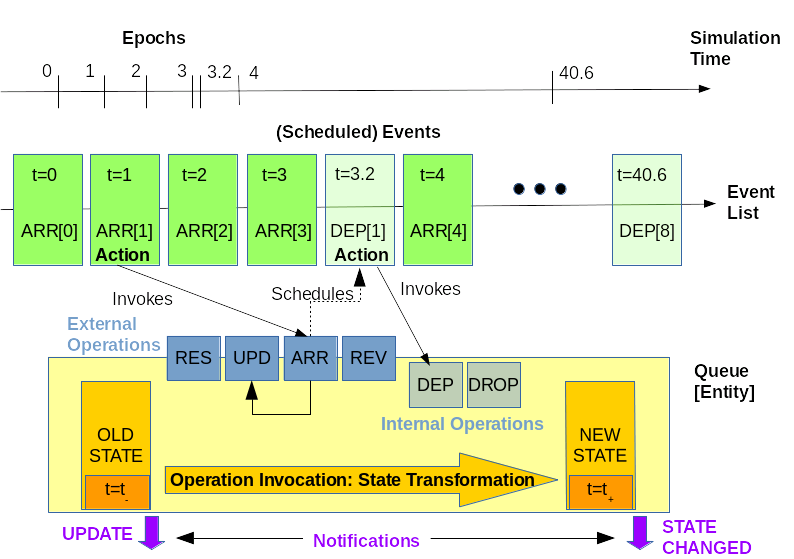
\includegraphics[width=\textwidth]{fig/SimpleSimulationOverview}
\end{figure}

In the top of the figure,
we show the simulation time and some of the epochs
from the example.
During a simulation run, the simulation time increases monotonically
as a function of "real time".
What this says is that the simulation time does not
"strictly decrease" in real time,
but at the same time,
that's pretty much the only requirement
on the relation between real time
and simulation time.
For instance,
processing the epochs between $t=0$ and $t=9$
may take several minutes in real time,
whereas epochs between $t=9$ and $t=100$
could be done in a mere second\footnote{
	This is not to say that is is impossible or even hard
	to let simulation time progress
	(roughly) at the same rate as real time,
	or at some scaled version of it.
	However, in discrete-event simulation,
	the relationship between real time and simulation time
	is generally considered unimportant.}

Below the simulation-time line,
we show the event list and some of the scheduled events
from the example.
The apparent equal distance between the events
is actually on pupose.
The event list is really not concerned with the
simulation-time differences between adjacent events.
No matter how large the time interval between an
event and its predecessor,
in between (basicaly) nothing happened:
There were not events,
and hence,
no state changes.
Going back to the figure,
we scheduled the arrival events ourselves
before processing the event list,
but we also see two "departure events"
we did not schedule.
In fact, these events were scheduled by the
queue, in response to previous events.
For instance, when job $1$ arrives at $t=1$ (simulation time),
it is taken into service immediately,
and after requesting the service time from job $1$ ($2.2$),
it schedules a {\em departure event\/} at $t=3.2$,
shown in a somewhat different color because we
did not schedule this ourselves (we are not even allowed to do so).
This shows an important aspect of the event list while processing it:
in general, the actions taken while processing the event list have
full freedom to schedule new events,
as long as they are not in the past.
This, admittedly, is not clear from the figure.
What is essential to remember is that a scheduled event
await its turn while the event list is being processed,
and the event list invokes the event's action
when it has processed all preceding events.

Assuming the event's action involves the queue in question,
we now turn our attention to the bottom part of the figure,
showing our queue from the example, the \lstinline|FCFS_B| queue.
We assume the arrival event at $t=1$ is processed by the event list,
and the net effect of this (i.e., the action of the event)
is the invokation of the arrival operation on the queue
(with the job $1$ as its argument).
As a result of this operation,
the state of the queue will transform,
and registered listeners to the queue will be informed
of the new state upon completion of the operation.
This, effectively, is the \lstinline|STATE CHANGED| notification.
In the figure this is shown with the right-pointing arrow at the bottom
from \lstinline|OLD STATE| to \lstinline|NEW STATE|,
and the \lstinline|STATE CHANGED| notification below that.

However, before doing anything,
the arrival operation invokes
the so-called \lstinline|UPDATE| operation,
which exposes the {\em old\/} state
to listeners and internally registered "hooks",
and, subsequently, increases the most essential state
property, the {\em last update time}.
By now, you should realize that
as the event list progresses in simulation time,
queues (or better, {\em entities\/})
that are not affected by the events processed
will not be bothered at all.
Yet a queue needs to assure that time-stamped operations
never lie in the past,
so they need to maintain a notion of simulation time themselves.
The importance of the \lstinline|UPDATE| notification
lies in {\em statistics gathering},
in which it is essential to know exactly
during which (non-trivial) intervals
the state of a queue did {\em not\/} change,
and the lenght of such intervals.
As long as you are not involved in statistics-gathering,
you can safely ignore these notifications,
otherwise,
you can find more details in Section \ref{chap:statistics}.

Once the \lstinline|UPDATE| operation has been
fulfilled, the \lstinline|ARR| (job arrival) operation,
in this particular case,
checks the number of jobs waiting,
and drops the arriving job if the number is $2$ ($=$\lstinline|B|)
by invoking the internal operation \lstinline|DROP|.
However, for job $1$ in the example,
it finds an empty waiting area,
and, in addition, no job being served at the server.
This means that the job is taking into service immediately
(the \lstinline|START| internal operation),
and since the required service time is non-zero,
the queue schedules a {\em departure event\/}
at $t=3.2$.
The departur event, in turn,
will invoke the internal \lstinline|DEP| (job departure)
event because of which the job
will eventually depart from the queueing system.

So, what more is there to say.
Well, we seem to have so called {\em external\/}
and {\em internal\/} operations,
the latter of which we cannot schedule ourselves
(departures, drops, $\ldots$).
In a way, the external operations allow us
to subject a queue to some kind of {\em workload\/}
consisting of arriving jobs
(as well as of, yet undescribed, other external operations on the queue).
The internal operations, on the other hand,
are always involved from within the queue itself,
either as a response to a scheduled event,
or as a response to an invocation of an external operation
in combination with a state condition
(e.g., the arrival of a job while $2$ jobs are already waiting
causes the internal \lstinline|DROP| operation to be invoked).

\section{The \texttt{Update} Operation}
\label{sec:guided:update}

In the previous section we introduced the
\lstinline|UPDATE| and \lstinline|STATE CHANGED|
notifications,
and explained that on a \lstinline|SimEntity|,
every state-change must be reported,
and that the \lstinline|UPDATE| notification
exposes the old state of the entity
for (for instance) statistics gathering.
However, there also exits an \lstinline|Update|
operation.
Its function is to set the \lstinline|LastUpdateTime|
state property of the entity.
The example shown in
Listing \ref{simExample1_update_main}
with output
shown in Listing \ref{simExample1_update_out}
demonstrates its use,
again using utility methods
for scheduling.
As the output shows,
there seems to be little use in the \lstinline|Update|
operation; it just updates the time at $t=8.5$ and $t=1000$.
The reason why you would ever want to use \lstinline|Update|
is a bit involved,
and deferred until Chapter \ref{chap:entities-queues-jobs}.
However, we included this example to demonstrate
that the end-time of the simulation can be
controlled through scheduling an \lstinline|Update|
operation.
In the next section, we will delve a little deeper
into the end-time of a simulation.

\begin{lstfloat}
	\begin{lstlisting}[
	caption={The use of the \texttt{Update} operation.},
	label=simExample1_update_main,
	basicstyle=\tiny]
	
	final SimEventList el = new DefaultSimEventList ();
	final int bufferSize = 2;
	final FCFS_B queue = new FCFS_B (el, bufferSize);
	queue.registerStdOutSimEntityListener ();
	for (int j = 0; j < 4; j++)
	{
	final double jobServiceTime = (double) 2.2 * j;
	final double jobArrivalTime = (double) j;
	final String jobName = Integer.toString (j);
	final SimJob job = new DefaultSimJob (null, jobName, jobServiceTime);
	SimJQEventScheduler.scheduleJobArrival (job, queue, jobArrivalTime);
	}
	SimEntityEventScheduler.scheduleUpdate (el, queue, 8.5);
	SimEntityEventScheduler.scheduleUpdate (el, queue, 1000.0);
	el.run ();
	
	\end{lstlisting}
\end{lstfloat}

\begin{lstfloat}
	\begin{lstlisting}[
	caption={The output of Listing \ref{simExample1_update_main}.},
	label=simExample1_update_out,
	basicstyle=\tiny]
	
	StdOutSimEntityListener t=0.0, entity=FCFS_B[2]: UPDATE.
	StdOutSimEntityListener t=0.0, entity=FCFS_B[2]: STATE CHANGED:
	=> ARRIVAL [Arr[0]@FCFS_B[2]]
	=> START [Start[0]@FCFS_B[2]]
	=> DEPARTURE [Dep[0]@FCFS_B[2]]
	StdOutSimEntityListener t=1.0, entity=FCFS_B[2]: UPDATE.
	StdOutSimEntityListener t=1.0, entity=FCFS_B[2]: STATE CHANGED:
	=> ARRIVAL [Arr[1]@FCFS_B[2]]
	=> START [Start[1]@FCFS_B[2]]
	=> STA_FALSE [StartArmed[false]@FCFS_B[2]]
	StdOutSimEntityListener t=2.0, entity=FCFS_B[2]: UPDATE.
	StdOutSimEntityListener t=2.0, entity=FCFS_B[2]: STATE CHANGED:
	=> ARRIVAL [Arr[2]@FCFS_B[2]]
	StdOutSimEntityListener t=3.0, entity=FCFS_B[2]: UPDATE.
	StdOutSimEntityListener t=3.0, entity=FCFS_B[2]: STATE CHANGED:
	=> ARRIVAL [Arr[3]@FCFS_B[2]]
	StdOutSimEntityListener t=3.2, entity=FCFS_B[2]: UPDATE.
	StdOutSimEntityListener t=3.2, entity=FCFS_B[2]: STATE CHANGED:
	=> DEPARTURE [Dep[1]@FCFS_B[2]]
	=> START [Start[2]@FCFS_B[2]]
	StdOutSimEntityListener t=7.6000000000000005, entity=FCFS_B[2]: UPDATE.
	StdOutSimEntityListener t=7.6000000000000005, entity=FCFS_B[2]: STATE CHANGED:
	=> DEPARTURE [Dep[2]@FCFS_B[2]]
	=> START [Start[3]@FCFS_B[2]]
	StdOutSimEntityListener t=8.5, entity=FCFS_B[2]: UPDATE.
	StdOutSimEntityListener t=14.200000000000001, entity=FCFS_B[2]: UPDATE.
	StdOutSimEntityListener t=14.200000000000001, entity=FCFS_B[2]: STATE CHANGED:
	=> DEPARTURE [Dep[3]@FCFS_B[2]]
	=> STA_TRUE [StartArmed[true]@FCFS_B[2]]
	StdOutSimEntityListener t=1000.0, entity=FCFS_B[2]: UPDATE.
	
	\end{lstlisting}
\end{lstfloat}

In summary:
\begin{itemize}
  \item Queues and jobs are collectively referred to as simulation {\em entities}.
  \item Simulation entities always start in a known type-specific {\em default state},
          also referred to their \lstinline|RESET STATE| upon construction
          and upon performing their \lstinline|RESET| operation.
  \item Simulation entities must always report any change to their state through
	  \lstinline|STATE CHANGED| notifications to registered {\em listeners}.
  \item Simulation entities only change their state
          as a result of the invocation of a well-defined
          {\em operation\/} on the entity.
        The operation can be external (like \lstinline-ARRIVAL-)
          or internal (like \lstinline-START-, \lstinline-DROP-, and \lstinline-DEPARTURE-).
  \item Any operation invocation takes zero (simulation) time to perform.
        Upon invocation of an operation, the new simulation time has to be supplied
          by the caller.
        With the exception of the \lstinline|RESET| operation,
          the new time provided must not be strictly smaller than the
          time of the previous invocation (of {\em any\/} operation).
  \item Before even starting the transformation from an old state into a new state,
	  simulation entities must always expose their {\em old\/} state
	  with a \lstinline|UPDATE| notification.
  \item Depending on the registered listener,
	  a simulation entity also fires {\em courtesy\/} notifications,
          revealing only a specific aspect of the state change.
        Courtesy notifications are {\em always\/} fired {\em after\/}
          the applicable \lstinline|STATE CHANGED| notification.
\end{itemize}

\section{Resetting Entities}

Every simulation entity (queue or job) supports the
external \lstinline-RESET- operation
that puts the entity into its {\em default\/} or
{\em reset\/} state.
It is the only operation that is allowed to
set {\em back\/} the time.
The new time on the entity is taken from the event list,
or to $-\infty$ if no event list is available.

The \lstinline-RESET- state of an entity depends
on the type of entity,
but it must be clearly specified.
It is, however, subject to strict rules,
as shown in Tables
\ref{resetStateSettings-queue}
and
\ref{resetStateSettings-job}.
For instance,
in the \lstinline|RESET| state,
a queue is empty (no jobs visiting).
The \lstinline|QueueAccessVacation| and
\lstinline|ServerAccessCredits|
properties will be decribed shortly
in the next sections.
In its \lstinline|RESET| state,
a job is not visiting any queue;
its \lstinline|Queue| propery is \lstinline|null|.
Beware however,
that queues are mandatorily attached to the event list,
whereas for jobs this is not required.
A queue will therefore set
the \lstinline|Queue| property to \lstinline|null|
for the jobs that it forcibly removes.

\begin{table}[h]
	\caption{Mandatory settings in the \texttt{RESET} state
		of a queue.}
	\label{resetStateSettings-queue}
	\begin{center}
		\begin{tabular}{|l|l|l|}
			\hline
			Property & Type & Default Value \\ \hline
			\lstinline|LastUpdateDate|      & \lstinline|double|      & From event list or $-\infty$.               \\ \hline
			\lstinline|Jobs|                & \lstinline|Set<SimJob>| & Empty set.                                  \\ \hline
			\lstinline|QueueAccessVacation| & \lstinline|boolean|     & \lstinline|false|.                          \\ \hline
			\lstinline|ServerAccessCredits| & \lstinline|int|         & \lstinline|Integer.MAX_VALUE| (==$\infty$). \\ \hline
			\lstinline|StartArmed|          & \lstinline|int|         & Depends on \lstinline|SimQueue| type.       \\ \hline
		\end{tabular}
	\end{center}
\end{table}

\begin{table}[h]
	\caption{Mandatory settings in the \texttt{RESET} state
		of a job.}
	\label{resetStateSettings-job}
	\begin{center}
		\begin{tabular}{|l|l|l|}
			\hline
			Property & Type & Default Value \\ \hline
			\lstinline|LastUpdateDate|      & \lstinline|double|      & From event list or $-\infty$.               \\ \hline
			\lstinline|Queue|               & \lstinline|SimQueue|    & \lstinline|null|.                           \\ \hline
		\end{tabular}
	\end{center}
\end{table}

\section{Summary of the \texttt{SimEntity} Interfaces}
\label{sec:guided:simentity-model}

In this section,
having seen almost all aspects of \lstinline|SimEntity|s,
\lstinline|SimJob|s,
and \lstinline|SimQueue|s,
we summarize their state and behavior.
We have two purposes in mind:
\begin{itemize}
	\item To present the material presented thus far in a format
	that allows you to assert your understanding
	of the fundamental concepts in \lstinline|jqueues|
	and \lstinline|jsimulation|.
	\item To present the interfaces in a compact overview format
	that can be used as a reference.
	Really, at this point we have covered almost every aspect
	of entities, queues, and jobs, and their listeners.
	The remainder of this Chapter will focus at some
	left-overs and an important class of queues
	named {\em composite queues}.
	The remainder of this entire book is really
	about explaining rigorously the abstract interfaces
	and the specific concrete types
	of queues (mostly), jobs and listeners,
	and about how you can build your own.
	In other words, the summary presented in this section
	is quite complete already,
	hence it is worth using as a reference.
\end{itemize}
